
\chapter{
    گونه‌های مختلف مسئله
}
\section{
    گونه‌های مختلف مسئله
}
پژوهش‌های گسترده ای روی مسئله‌ی کدگذاری اندیس منعطف انجام شده است. یکی از روش‌های پژوهشی تعریف گونه‌های جدیدی از مسئله با استفاده از قیدهای جدید است.

در این فصل با ۴ گونه دیگر آشنا می‌شویم که هر کدام با در نظر گرفتن قیدی متفاوت، مسئله‌ای متفاوت تعریف می‌کنند که کاربردهای مختلفی دارند. همان طور که با منعطف کردن نیازمندی گیرنده‌ها در مسئله‌ی کدگذاری اندیس مسئله‌ی کدگذاری اندیس منعطق را تعریف کردیم، در بخش اول با افزایش میزان منعطف بودن گیرنده‌ها، مسئله‌ی 
\transf{کدگذاری اندیس بسیار منعطف}{very pliable index coding}
 تعریف می‌شود. در بخش دوم با در نظر گرفتن ترجیح‌های مختلف گیرنده‌ها برای یافتن پیا‌های مختلف مسئله‌ی
 \transf{کدگذاری اندیس منعطف ترجیحی}{Preferential Pliable Index Coding}
 را تعریف می‌کنیم. در بخش سوم با حذف فرستنده‌ی مرکزی، گیرنده‌ها به صورت محلی اطلاعات خود را به اشتراک می‌گذارند و مسئله‌ی
 \transf{کدگذاری اندیس منعطف غیرمتمرکز}{Decentralized Pliable Index Coding}
 را تعریف میکنیم. در بخش نهایی با در نظر گرفتن محرمانگی برای پیام‌ها به این صورت که هر گیرنده نتواند بخشی از پیام‌هایی که ندارد را پیدا کند مسئله‌ی
 \transf{کدگذاری اندیس منعطف خصوصی}{Private Pliable Index Coding}
 را تعریف می‌کنیم.
 
 هدف از این فصل، آشنایی به گونه‌های مختلف مسئله‌ی کدگذاری اندیس منعطف است تا افق دید ما برای پژوهش‌های مختلف افزایش بیابد و همچنین داشتن مروری کامل در این رساله بر تلاش‌های مختلف برای بررسی و یافتن گزاره‌های جدید است.

\section{کدگذاری اندیس بسیار منعطف}
برای حل مسئله کدگذاری اندیس از روی گراف اطلاعات جانبی، ابتدا مشخص میکنیم که به ازای هر انتخابی از پیام‌ها چه پیام‌هایی را فرستنده ارسال میکنید به طوری که هر گیرنده پیام مورد نظرش را بازیابی کند. در کدگذاری اندیس منعطف از روی گراف اطلاعات جانبی ابتدا برای هر گیرنده مشخص میکنیم که چه پیامی را قرار از بازیابی کند. سپس به ازای هر انتخاب پیام‌ها، پیام‌هایی که فرستند باید ارسال کند مشخص میکنیم و در نهایت هر گیرنده پیامی که برایش انتخاب شده است را بازیابی می‌کند. در مسئله کدگذاری اندیس بسیار منعطف مانند کدگذاری اندیس معمولی از روی گراف اطلاعات جانبی پیام‌هایی که سرور باید ارسال کند را مشخص میکنیم. سپس هر گیرنده بر اساس اطلاعات جانبی خود و پیام‌های دریافت شده خواهد توانست حداقل یکی از پیام‌هایی که از قبل نداشته است را بازیابی کند. در واقع اینکه کدام پیام را بازیابی کند بستگی به اطلاعات جانبی او و پیام‌های دریافتی از فرستنده دارد.

این مسئله توسط اونگ و ولامبی در
\cite{verypliable}
معرفی شده است. آن‌ها نشان می‌دهند که منعطف کردن بیشتر گیرنده‌ها برای حالت خطی هیچ بهبودی در کران‌ها ایجاد نمیکند ولی برای حالت کلی کران‌های اکیدا بهتری ایجاد می‌کند. همچنین برای حالتی که اندازه پیام‌ها متناهی است نسبت به حالتی که به صورت حدی بزرگ باشد نرخ‌هایی بهتری کسب پیدا می‌کنند. همچنین نشان می‌دخند که نرخ بهینه برای این مسئله حداقل یک است. همچنین روشی برای ساخت کدهای بسیار منعطف با الفبای بزرگتر از روی کدهای بسیار منعطف با الفبای کوچک تر می‌سازند.

برای مثال فرض کنید سه پیام داریم و سه گیرنده که هر کدام یکی از پیام‌ها را به عنوان اطلاعات جانبی می‌داند. در این حالت برای مسئله‌ی کدگذاری اندیس بسیار متعطف می‌توانیم پیام‌های مختلف را به صورت زیر دسته بندی کنیم:
\begin{figure}[H]
	\centering
	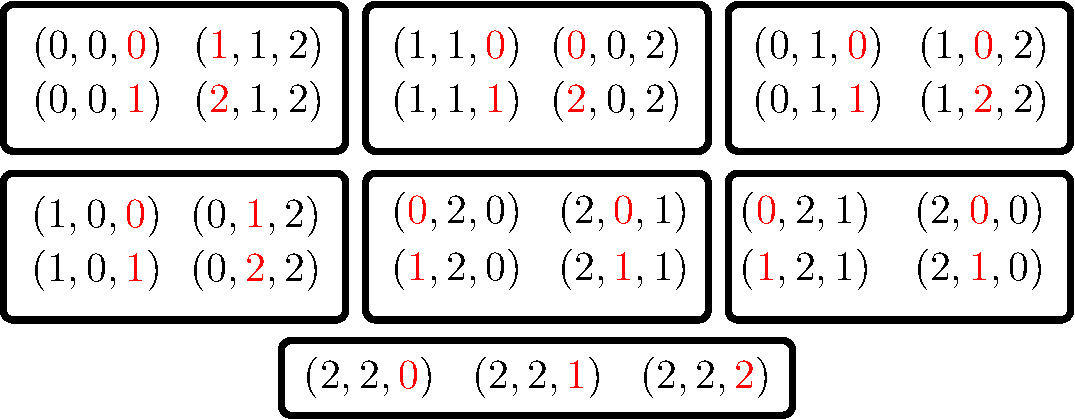
\includegraphics[width=8cm]{figs/chapter4/Alpha3}
	\caption{
		کدگذاری بسیار منعطف با نرخ بهینه برای
		$m=3$, 
		$\mathbb{U} = \big\{ \{1\}, \{2\}, \{3\} \big\}$,
		 $k=3$.
		 }
	\label{fig:eg:0}
\end{figure}
حال برای مثال اگر پیام‌ها از دسته اول باشند(فرستنده اندیس این دسته را ارسال کند) در این صورت گیرنده ای که پیام دوم را از قبل می‌اند به صورت زیر پیام جدیدی را پیدا میکند:
$$X_2 = 0 \Rightarrow X_1 = 0$$
و
$$X_2 = 1 \Rightarrow X_3 = 2$$

ابزار اصلی استفاده شده در این مقاله نظریه اطلاعات است. تقریبا تمام قضایا با محاسبه آنتروپی اثبات می‌شوند. همچنین کران پایین با استفاده از
 کدهای ام‌دی‌اس
 ~\ref{def:mds}
به دست می‌آید.


\section{کدگذاری اندیس منعطف ترجیحی}
در مسئله‌های کدگذاری اندیس و کدگذاری اندیس منعطف و بسیار منعطف پیام‌ها برای گیرنده‌ها ارجحیتی بر یک دیگر ندارند بلکه صرفا بازیابی هر پیامی که گیرنده از پیش نداشته باشد کافی است. بایرنه اونگ صادقی و دیگران در
\cite{byrne2023preferential}
با افزودن ترجیحات گیرنده‌ها بر روی پیام‌ها مسئله‌ی کدگذاری اندیس منعطف ترجیحی را تعریف کرده اند. هدف آن‌ها پیدا کردن کدهایی است که به صورت هم‌زمان نرخ ارسال و رضایت کلی گیرنده‌ها را بهبود ببخشد. برای این کار آن‌ها به دنبال مرز	پارتو
\ref{def:Pareto-boundary}
 در فضای جواب‌ها میگردند.
 
 یک راه‌حل 
 \transf{
 بروت‌فورس}{
  brute-force
  }
 برای مسئله‌ی کدگذتری اندیس منعطف این است که برای هر گیرنده انتخاب کنیم که کدام پیام را می‌خواهد بازیابی کند و بدین صورت مسئله را به مسئله‌ی کدگذاری اندیس تبدیل و حل کنیم و بین تمام انتخاب‌های مختلف مقدار بهینه را انتخاب کنیم.  راه‌حل های
 \transf{
 ابتکاری
 }{
 heuristic
 }
 در مسئله‌ی کدگذاری اندیس منعطف به جای یک 
 \transf{
 جست‌وجوی جامع
 }{
 exhaustive search
 }
به دنبال 
\transf{
زیرکدهایی
}{sub-codes}
هستند که در هر تکرار تعداد
\transf{ 
ماکسیمالی
}{
maximal
}
از گیرنده‌ها را ارضا کنند و این کار را تکرار میکنند تا زمانی که کل گیرنده‌ها ارضا شوند. به طور مشابه برای کدگذاری اندیس منعطف ترجیجی میتوان با یک جست‌وجوی جامع برای تمام حالت‌های مختلف کدگذاری مقدار رضایت کلی گیرنده‌ها و طول کد را پیدا کرد که از نظر پیچیدگی محاسبه اصلا قابل قبول نیست. بایرنه و همکاران در مقاله خود یک الگوریتم ابتکاری ارائه می‌دهند که در هر تکرار به جای اینکه تنها تعداد گیرنده‌ها را حداکثر کند تابع هدفی را حداکثر کند که با دقت موازنه ای بین هر دو معیار برقرار کند سپس با نتایج عددی نشان می‌دهند که الگوریتم را می‌توان برای هر کدام از معیار ها بهینه کرد و خروجی نزدیک به مرز پارتو به دست اورد.
\begin{definition}
	ماتریس ترجیح
	$\boldsymbol{P}$ 
	برای یک مسئله‌ی کدگذاری اندیس منعطف ترجیحی یک ماتریس
	 $n\times m$
	 است که:
	\begin{equation}
		\boldsymbol{P} = [P_{i,j}]_{n\times m},
	\end{equation}
	به طوری که
	 $P_{i,j}\in\mathbb{R}\cup\{\infty\}$ 
	 ترجیح گیرنده‌ی
	 ~$i$
	 برای پیام
	  $X_j$
	  است.
	اگر یک پیام جز اطلاعات جانبی یک گیرنده باشد مقدار ترجیح آن بی‌نهایت است.
	
	در واقع ترجیح کمتر به معنی ارجحیت آن پیام است.
\end{definition}

مثال:
\begin{equation}
	\boldsymbol{P} = 
	\begin{bmatrix}
		2 & \infty & 1 &\infty & 2\\
		\infty & 1 & 2 & 1 & \infty \label{eq:ppicod-instance}
	\end{bmatrix}.
\end{equation}
\begin{figure}[H]
	\centering
	
\includegraphics[width=0.2\linewidth]{figs/chapter4/ppgraph.pdf}
	\caption{}
	\label{fig:ppgraph}
\end{figure}
در واقع برعکس مدل سازی گرافی اصلی که یال برای نشان دادن اطلاعات جانبی بود اینجا برای نشان دادن اطلاعات جانبی نبودن است.
برای اینکار از الگوریتم زیر استفاده می‌کنند:
\begin{latin}

\begin{algorithm}[H]
	\caption{PrGrCov($G,\alpha,\boldsymbol{\eta}$)}\label{alg:pr-grcov}
	\begin{algorithmic}[1]
		\State Inputs: A PPICOD graph $G=(\mathbb{U}, [1:m], E, w)$ and parameters $\alpha$, $\boldsymbol{\eta}$
		\State $\mathcal{C} \gets \emptyset$
		\State $\mathsf{SAT} \gets \emptyset$ 
		\While{$|\mathsf{SAT}| \neq n$}
		\State $\textrm{maximal} \gets \code{False}$
		\State $\mathcal{S} \gets \emptyset$
		\While{$\textrm{maximal} = \code{False}$}
		\State $\textrm{maximal} = \code{True}$
		\State Randomly pick $j^* \in \arg \max_{j \in [1:m] \setminus \mathcal{S}} f(\mathcal{S} \cup \{j\})$
		\If{$f(\mathcal{S} \cup \{j^*\}) > f(\mathcal{S})$}
		\State $\textrm{maximal} \gets \code{False}$
		\State $\mathcal{S} \gets \mathcal{S} \cup \{j^*\}$
		\EndIf
		\EndWhile
		\State $\mathsf{SAT} \gets \mathsf{SAT} \cup W_1(\mathcal{S})$
		\State $\mathcal{C} \gets \mathcal{C} \cup \{\mathcal{S}\}$
		%\State \% Remove outgoing edges from $W_1(\mathcal{S})$:
		\State $E \gets E \setminus \{ (u,v) \in E: u \in W_1(\mathcal{S})\}$
		\EndWhile
		\State Output: $\mathcal{C}$
	\end{algorithmic}
\end{algorithm}
\end{latin}

پارامتر 
$\alpha$
در این الگوریتم برای بهینه کردن خروجی با افزایش رضایت کلی و یا افزایش نرخ کد استفاده میشود. با افزایش 
$\alpha$
تعداد گیرنده‌هایی که ارضا می‌شوند در هر تکرار، به کد با طول کمتر می‌انجامد. در شکل زیر تاثیر این پارامتر را می‌بینید.
\begin{figure}[H]
	\centering
	%\subcaptionbox{$s$ versus $\alpha$}
	{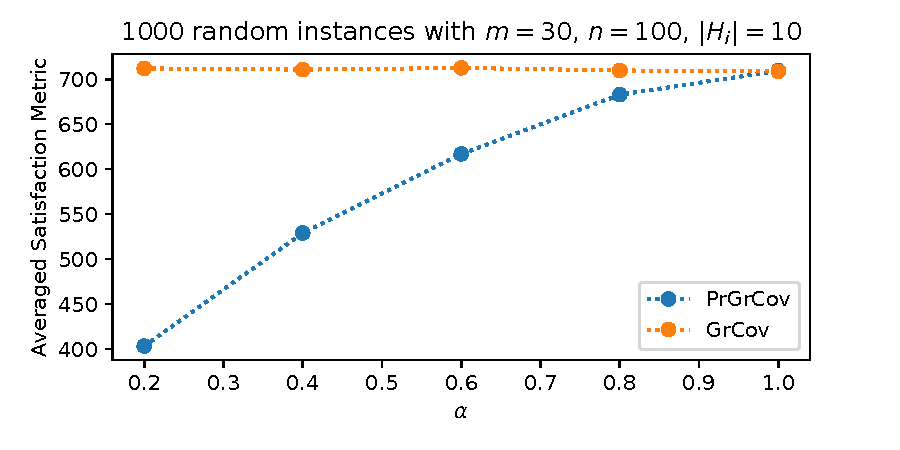
\includegraphics[width=0.4\linewidth]{figs/chapter4/cost_alpha_grcov_prgrcov.pdf}\vspace{-2ex}}
	%\subcaptionbox{$\ell$ versus $\alpha$}
	{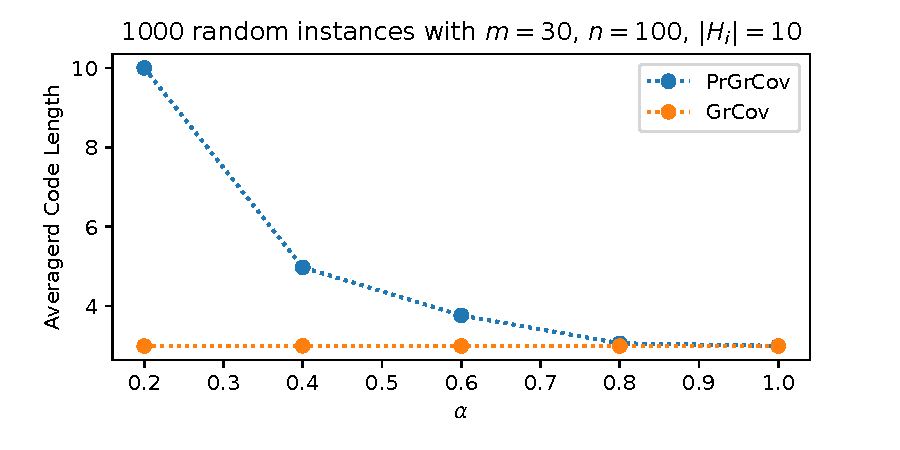
\includegraphics[width=0.4				\linewidth]{figs/chapter4/code_length_alpha_grcov_prgrcov.pdf}\vspace{-2ex}}
	\caption{The effect of $\alpha$ on satisfaction index and code length averaged over 1000 randomly generated PPICOD problems.}\label{fig:alpha}
\end{figure}

\section{کدگذاری اندیس منعطف غیرمتمرکز}
ساختار مسائل مشتق شده از کدگذاری اندیس به طور کلی شامل یک فرستنده‌ی مرکزی است که با دانستن پیام‌ها و گراف اطلاعات جانبی با ارسال تعدادی پیام باعث می‌شود گیرنده‌ها به پیام‌های جدیدی دست بیابند. لیو و تونینتی در
\cite{paper:Decentralized}
با حذف فرستنده‌ی مرکزی و ارسال تعدادی پیام توسط خود گیرنده‌ها بازیابی پیام‌های جدید را به صورت غیرمتمرکز دنبال می‌کنند. در این نسخه هر گیرنده تعدادی پیام ارسال می‌کند که تمام گیرنده‌های دیگر دریافت میکنند یعنی به جای یک تابع کدگذاری به هر گیرنده یک تابع کدگذاری اختصاص داده می‌شود که بر اساس اطلاعات جانبی تعداد پیام برای بقیه گیرنده‌ها ارسال میکند. همچنین توابع کدگشایی هم برای هر گیرنده با استفاده از اطلاعات جانبی و پیام‌های دریافتی از بقیه گیرنده‌ها پیام جدید را بازیابی می‌کنند.

این مسئله را در واقع میتوان حالت خاصی از مسئله کدگذاری اندیس توزیع شده
\cite{9022912}
دانست. به این صورت که به تعداد گیرنده‌ها فرستنده وجود دارد و هر فرستند نظیر یک گیرنده است. هر فرستنده به اطلاعات جانبی گیرنده نظیر خود دسترسی دارد. هدف کاهش تعداد استفاده از کانال ارتباطی است به گونه ای که تمام گیرنده ها پیامی جدید را بازیابی کنند.

لیو و همکاران در این مقاله به دلیل پیچیدگی مسئله فقط روی دو حالت خاص آن کار می‌کنند. برای 
$m$
پیام و مجموعه‌ی
$S = \{s_{min}, s_{min }+ 1, \ldots, s_{max}\}$
مسئله‌ی 
\lr{consecutive complete–S PICOD(t)}
را به این صورت تعریف می‌کنیم. به ازای تمام حالت‌های اطلاعات جانبی ممکن از اندازه
$s \in S$
یک گیرنده در نظر میگیریم یعنی
$n = \sum\limits_{s \in S} \binom{m}{s}$
گیرنده خواهیم داشت. همچنین مسئله‌ی
\lr{complement-consecutive complete–S PICOD(t)}
را هم بر به طور مشابه برای مجموعه
$S = \{0, \ldots, m - t\} \setminus \{s_{min}, \ldots, s_{max}\}$
تعریف می‌کنیم.

در این مقاله نیز از نظریه اطلاعات و ترکیبیات برای اثبات قضایا استفاده می‌شود و با استفاده از کدهای ام‌دی‌اس نیز کد با کران بهینه را می‌سازند. قضیه اصلی ای که در این مقاله اثبات می‌شود در رابطه با طول کد های غیرمتمرکز است:
\begin{theorem}[consecutive]
	%[Optimal code-length for the decentralized consecutive complete--$S$ PICOD$(\cardi)$ with $m$ messages]
	\label{thm:consecutive_s}
	برای مسئله‌ی
	\lr{decentralized complete--$S$ PICOD$(\cardi)$}
	با
	$m$ 
	پیام و
	  $S=[\smin:\smax]$
	  برای یک
	  $0\leq \smin \leq \smax \leq m-\cardi$
	  طول کد بهینه برابر است با:
	\begin{align}
		\ell^{\star}=\begin{cases}
			\frac{\binom{m}{m-\cardi}}{\binom{m}{m-\cardi}-1}  \cardi, \quad \smax=\smin=m-\cardi,\\
			\min\{\smax+\cardi, m-\smin\}, \quad \text{otherwise.}
		\end{cases}
		\label{eq:thm:consecutive_s}
	\end{align}
\end{theorem}


\begin{theorem}[complement-consecutive]
	%[Optimal code-length for the decentralized complement-consecutive complete--$S$ PICOD$(\cardi)$  with $m$ messages]
	\label{thm:complement_consecutive_s}
	برای مسئله‌ی
\lr{ decentralized complete--$S$ PICOD$(\cardi)$}
با
 $m$ 
 پیام
 و
 $S=[0:m-\cardi]\backslash [\smin:\smax] = [0:\smin-1]\cup[\smax+1:m-\cardi]$
 برای یک
 $0 < \smin \leq \smax < m-\cardi$
 طول کد بهینه برابر است با
	\begin{align}
		\ell^{\star}=\min\{m,|S|+2\cardi-2\}.
		\label{eq:thm:complement_consecutive_s}
	\end{align}
\end{theorem}

\section{کدگذاری اندیس منعطف خصوصی}
مسئله‌ی امنیت و حریم خصوصی در کدگذاری اندیس از جنبه‌های مختلف بررسی شده است. دائو و همکاران در
\cite{6166891}
یک گیرنده دیگر نیز وجود دارد که دسترسی محدودی به اطلاعات جانبی و پیام‌های ارسال شده توسط فرستنده دارد و هدف این است که نتواند پیام جدیدی را بازیابی کند. کارموزه و همکاران(که شامل فرگولی نیز میشود) در
\cite{8006988}
پیام‌های ارسال شده توسط فرستنده باید به گونه ای باشد که هر گیرنده بتواند پیام مورد نظر خود را بازیابی ولی نتواند هیچ اطلاعاتی راجع به اطلاعات جانبی و پیام‌های مورد نظر بقیه گیرنده‌ها کسب کند که شبیه به ایده‌ی
\transf{مسئله‌ی بازیابی اطلاعات خصوصی}{private
	information retrieval problem}
	مطرح شده در
\cite{7889028}
است.
نارایانا و همکاران در
\cite{9627083}
مسئله‌ی کدگذاری اندیس خصوصی را به این شکل صورت بندی می‌کنند که هر گیرنده فقط پیام‌های مورد نظر خودش را بازیابی کند و هیچ پیام دیگری را نتواند بازیابی کند. ساسی و راجان در
\cite{sasi2019pliable}
این تعریف را برای کدگذاری اندیس منعطف تعمیم می‌دهند. اما فقط برای حالتی که ساختار اطلاعات جانبی دایره‌ای است و هر گیرنده تنها و فقط تنها یک پیام را می‌تواند بازیابی کند.

لیو و تانینوتی در 
\cite{8989161}
این تعریف را بسط داده و کران‌های قابل دستیابی به دست می‌اورند.

تعریف کدگذاری اندیس منعطف خصوصی مشابه تعریف کدگذاری اندیس منعطف است همراه با شرط زیر:
گیرنده‌ی
$u_j$
نمیتواند هیچ پیامی به جز
 $\cardi$ 
 پیامی که قرار است بازیابی کند را بازیابی کند.